
\chapter{Director}
\label{sec:director}

\section{Problematica}
\label{sec:problema}
Descripcion del problema que se pretende mitigar con el lenguaje

El presente trabajo pretende presentar una herramienta que aplique los
conceptos vistos en la \texttt{Sección \ref{sec:mdsd}} referentes a MDSD,
focalizando el uso de modelos UML, tales restricciones determinan que se siguen
los patrones relacionados a MDA como se acotó en la
\texttt{Sección \ref{sec:arquitectura_dirigida_por_modelos}}, como se menciona
en la sección para MSDS, para la implementación de tales técnicas, uno de los
requisitos es la definición de un Lenguaje Específico de Dominio, (tratado en
la \texttt{Sección \ref{sec:dsl}}).

Director, proveera de un lenguaje especifico de dominio que permite el modelado de
sistemas de información orientados a objetos, en esta primera iteración del
mismo, se pretende incluir las entidades utilizadas en la realización de
gráficas de Diagramas de Clase pertenecientes a la familia de Diagramas UML.

\section*{Estructura del Lenguaje}
A continuación, se presentarán en diferentes secciones los componentes que
hacen al lenguaje, estos se ubicaran según el nivel de dependencia de cada uno
con respecto a los demás componentes, de esta manera, compartimentando la
responsabilidad se hace a una explicación mas simplificada de la herramienta.

Se pueden esperar, para cada sección que describe a un elemento del lenguaje,
las siguientes notaciones que formalizan a la propuesta del presente
documento: \texttt{Gramática libre de contexto en formato BNF (Backus-Naur)},
\texttt{Expresiones Regulares}, \texttt{Autómatas Finitos}.

\section{Palabras Reservadas}
\label{sec:palabrasreservadas}

Aquí se describirán las palabras utilizadas como tokens en el lenguaje
propuesto, estas permiten, desde el establecimiento de relaciones
entre entidades de un modelo, hasta la habilidad de indicar el tipo de devolución
de un método. A continuación se proporciona una lista de palabras reservadas
con su correspondiente explicación:

\begin{description}[align=right,labelwidth=2.5cm]

\item [class] Esta palabra se utiliza como token para la definición de una clase,
	es un componente de alto nivel dentro del lenguaje.

	Ejemplo:
		\begin{lstlisting}
		class Persona {
			...
			}
		\end{lstlisting}

\item [relationships] Palabra utilizada para establecer relaciones inter-clase
	dentro de un modelo, esta es una entidad de alto nivel en el lenguaje que
	permite la relación mediate \textit{herencia}, \textit{asociación}, etc,
	entre clases de un modelo.

	Ejemplo:
		\begin{lstlisting}
		...
		relationships {
			...
			}
		\end{lstlisting}

\item [void] Token que permite establecer el tipo de la devolución de un
	método, éste indica que el método no hace ninguna	devolución.

	Ejemplo:
		\begin{lstlisting}
		  ...
			<visibilidad> metodo():void
			...
		\end{lstlisting}

\item [integer] Token que permite indicar el tipo de dato devuelto por un metodo, o
	el tipo de dato de un atributo. Hace referencia al tipo de
	datos entero; equivalente en un lenguaje como Java, \texttt{int}.

	Ejemplo:
		\begin{lstlisting}
		  ...
			<visibilidad> atributo:integer
			<visibilidad> metodo():integer
			...
		\end{lstlisting}

\item [double] Token que permite indicar el tipo de dato devuelto por un metodo, o
	el tipo de dato de un atributo. Hace referencia al tipo de
	datos doble; equivalente en un lenguaje como Java, \texttt{double}.

	Ejemplo:
		\begin{lstlisting}
		  ...
			<visibilidad> atributo:double
			<visibilidad> metodo():double
			...
		\end{lstlisting}

\item [float] Token que permite indicar el tipo de dato devuelto por un metodo, o
	el tipo de dato de un atributo. Hace referencia al tipo de
	datos con presición flotante; equivalente en un lenguaje como Java,
	\texttt{float}.

	Ejemplo:
		\begin{lstlisting}
		  ...
			<visibilidad> atributo:float
			<visibilidad> metodo():float
			...
		\end{lstlisting}

\item [long] Token que permite indicar el tipo de dato devuelto por un metodo, o
	el tipo de dato de un atributo. Hace referencia al tipo de
	datos largo; equivalente en un lenguaje como Java, \texttt{long}.

	Ejemplo:
		\begin{lstlisting}
		  ...
			<visibilidad> atributo:long
			<visibilidad> metodo():long
			...
		\end{lstlisting}

\item [boolean] Token que permite indicar el tipo de dato devuelto por un metodo, o
	el tipo de dato de un atributo. Hace referencia al tipo de
	datos booleanos; equivalente en un lenguaje como Java, \texttt{boolean}.

	Ejemplo:
		\begin{lstlisting}
		  ...
			<visibilidad> atributo:boolean
			<visibilidad> metodo():boolean
			...
		\end{lstlisting}

\item [string] Token que permite indicar el tipo de dato devuelto por un metodo, o
	el tipo de dato de un atributo. Hace referencia al tipo de
	datos de cadena de caracteres ; equivalente en un lenguaje como Java, \texttt{String};
	equivalente en C, \texttt{char[N]}.

	Ejemplo:
		\begin{lstlisting}
		  ...
			<visibilidad> atributo:string
			<visibilidad> metodo():string
			...
		\end{lstlisting}

\item [char] Token que permite indicar el tipo de dato devuelto por un metodo, o
	el tipo de dato de un atributo. Hace referencia al tipo de
	datos de caracter; equivalente en un lenguaje como Java, \texttt{char}.

	Ejemplo:
		\begin{lstlisting}
		  ...
			<visibilidad> atributo:char
			<visibilidad> metodo():char
			...
		\end{lstlisting}

\item [list] Token que permite indicar el tipo de dato devuelto por un metodo, o
	el tipo de dato de un atributo. Hace referencia a una
	estructura de colección reminiscente a las listas; equivalente en un lenguaje
	como Java, \texttt{List}.

	Ejemplo:
		\begin{lstlisting}
		  ...
			<visibilidad> atributo:list<tipo>
			<visibilidad> metodo():list<tipo>
			...
		\end{lstlisting}

\item[set] Token que permite indicar el tipo de dato devuelto por un metodo, o
	el tipo de dato de un atributo. Hace referencia a una
	estructura de colección reminiscente a los conjuntos; equivalente en un lenguaje
	como Java, \texttt{Set}.

	Ejemplo:
		\begin{lstlisting}
		  ...
			<visibilidad> atributo:set<tipo>
			<visibilidad> metodo():set<tipo>
			...
		\end{lstlisting}

\item [public] Esta palabra permite establecer la visibilidad de un elemento
	dentro del modelo, este elemento puede ser un atributo o una clase.

	Ejemplo:
		\begin{lstlisting}
		  ...
			public atributo:<tipo>
			public metodo():<tipo>
			...
		\end{lstlisting}

\item [private] Esta palabra permite establecer la visibilidad de un elemento
	dentro del modelo, este elemento puede ser un atributo o una clase.

	Ejemplo:
		\begin{lstlisting}
		  ...
			private atributo:<tipo>
			private metodo():<tipo>
			...
		\end{lstlisting}

\item [protected] Esta palabra permite establecer la visibilidad de un elemento
	dentro del modelo, este elemento puede ser un atributo o una clase.

	Ejemplo:
		\begin{lstlisting}
		  ...
			protected atributo:<tipo>
			protected metodo():<tipo>
			...
		\end{lstlisting}

\item[derivate] Esta palabra permite establecer la visibilidad de un elemento
	dentro del modelo, este elemento puede ser un atributo o una clase.

	Ejemplo:
		\begin{lstlisting}
		  ...
			derivate atributo:<tipo>
			derivate metodo():<tipo>
			...
		\end{lstlisting}

\item [package] Esta palabra permite establecer la visibilidad de un elemento
	dentro del modelo, este elemento puede ser un atributo o una clase.

	Ejemplo:
		\begin{lstlisting}
		  ...
			package atributo:<tipo>
			package metodo():<tipo>
			...
		\end{lstlisting}

\item [@id] Esta palabra se utiliza como un modificador en el ambito de
	los atributos de clase, este permite brindar información extra acerca del
	atributo en cuestión, en específico, este indica que el atributo es parte del
	identificador de la clase que lo posee.

	Ejemplo:
		\begin{lstlisting}
		  ...
			<visibilidad> atributo:<tipo>{@id}
			...
		\end{lstlisting}

\item [@readOnly] Esta palabra se utiliza como un modificador en el ambito de
	los atributos de clase, este permite brindar información extra acerca del
	atributo en cuestión, en específico, este indica que el atributo solo podra
	ser accedido para lectura una vez se haya guardado.

	Ejemplo:
		\begin{lstlisting}
		  ...
			<visibilidad> atributo:<tipo>{@readOnly}
			...
		\end{lstlisting}

\item [@sequence] Esta palabra se utiliza como un modificador en el ambito de
	los atributos de clase, este permite brindar información extra acerca del
	atributo en cuestión, en específico, este indica que el valor que tome el
	atributo sigue una secuencia.

	Ejemplo:
		\begin{lstlisting}
		  ...
			<visibilidad> atributo:<tipo>{@sequence}
			...
		\end{lstlisting}

\item [@unique] Esta palabra se utiliza como un modificador en el ambito de
	los atributos de clase, este permite brindar información extra acerca del
	atributo en cuestión, en específico, este indica que el atributo no tiene
	duplicados.

	Ejemplo:
		\begin{lstlisting}
		  ...
			<visibilidad> atributo:<tipo>{@unique}
			...
		\end{lstlisting}

\end{description}


\section{Símbolos Especiales}
\label{sec:simbolosespeciales}

% introduccion a los simbolos especiales
En Director, varios de los símbolos especiales permiten sacar provecho de las
propiedades gráficas de UML para la confección del modelo, por ejemplo, se
implementan símbolos que representan una contraparte en las palabras reservadas
para la descripción de algún método/atributo. En el \texttt{Cuadro
\ref{c:s_especiales}} se presentan los símbolos que componen al lenguaje y una
breve explicación de cada uno de ellos.

\begin{table}[H]
\centering
\caption{Símbolos especiales}
\begin{tabular}{c p{9cm} }
\hline
	Símbolo & Descripción \\ \hline
	+ & Visibilidad de un método/atributo, equivalente a public\\
	- & Visibilidad de un método/atributo, equivalente a private\\
  \# & Visibilidad de un método/atributo, equivalente a protected\\
	/ & Visibilidad de un método/atributo, equivalente a derivate\\
$\sim$ & Visibilidad de un método/atributo, equivalente a package\\
	: & Permite la asignación de un tipo de dato a un método/atributo\\
$\#\#$ & Comentarios de línea dentro del modelo \\
$\#\{$ & Inicio comentarios multilínea dentro del modelo\\
$\}\#$ & Fin comentarios multilínea dentro del modelo\\
$\# +$ & Definición de metainformación para el modelo\\
$//$ & Comentario de línea para el código resultante del modelo\\
$/*$ & Inicio comentarios multilínea para el codigo resultante del modelo\\
$*/$ & Fin comentarios multilínea para el codigo resultante del modelo\\ \hline
\end{tabular}
\label{c:s_especiales}
\end{table}


\section{Método}
\label{sec:metodo}
Al igual que los atributos, los metodos, son componentes dentro del diagrama de
clases que ayudan a la manipulación de los datos, estos brindan el
comportamiento que es propio al objeto. El lenguaje presentado permite definir
métodos de la siguiente manera:

\begin{lstlisting}[caption={BNF - Método}, basicstyle=\footnotesize\ttfamily]
  <metodo>::=<visibilidad><nombre>"("<parametro>")" ":"<tipo>
  <metodo>::=<visibilidad><nombre>"("<parametros>")" ":"<tipo>
\end{lstlisting}

En donde se puede decir que \texttt{parametro(s)} se define de la siguiente
manera:

\begin{lstlisting}[basicstyle=\footnotesize\ttfamily]
  <parametro> ::= <nombre> ":" <tipo>
\end{lstlisting}

\begin{lstlisting}[basicstyle=\footnotesize\ttfamily]
  <parametros> ::= <parametro> | <parametros>
\end{lstlisting}

Director, está dotado de la capacidad para tratar los casos triviales del
manejo de los datos dentro de un objeto, estos casos triviales corresponden a
situaciones en las cuales una de las necesidades de comportammiento para un
objeto viene dado por la urgencia de agregar algún mecanismo que permita
acceder a los atributos del mismo, las acciones comunes de acceso a estos
atributos son las siguientes: definir el valor de un atributo y obtener el
valor de ese atributo, las cuales son solucionadas con los \texttt{setters}
y los \texttt{getters}.

Director, no requiere que se definan explicitamente estos métodos, éste los
genera de manera automática.

Teniendo en cuenta el ejemplo mencionado en la \texttt{Seccion
\ref{sec:atributo}}, Director automáticamente generaría los siguientes métodos
para el lenguaje Java:

\begin{lstlisting}[language=Java, basicstyle=\footnotesize\ttfamily,
label=lst:drt_java_metodo, caption={Java - Generación \texttt{Fragmento \ref{sec:atributo}}}]
  ...
	public String get_nombre(){
		return this.nombre;
		}

	public void set_nombre(String nombre){
		this.nombre = nombre;
		}

	public String get_apellido(){
		return this.apellido;
		}

	public void set_apellido(String apellido){
		this.apellido = apellido;
		}

	public String get_DNI(){
		return this.DNI;
		}

	public void set_DNI(String DNI){
		this.DNI = DNI;
		}
	...
\end{lstlisting}

De todos modos, es posible indicar otros metodos que se deseen incluir en el
modelo. Si agregaramos algun $metodo\_generico$ al ejemplo con el que se viene
trabajando, la lista de atributos y modelos quedaría definida de la siguiente
manera.

\begin{lstlisting}[caption={Director - Declaración de Método}, label=lst:drt_java_modelo_metodo_generico]
	private nombre:string
	private apellido:string
	private DNI:string
	public metodo_generico():void
\end{lstlisting}

Lo que resultaria en la generación del ``esqueleto'' necesario para la
implementación de dicho método. Tomando como base lo que ya se hizo en
el \texttt{Fragmento \ref{lst:drt_java_metodo}}, se le agregaría:

\begin{lstlisting}[caption={Java - Generación metodo\_generico agregado en
\texttt{Fragmento \ref{lst:drt_java_modelo_metodo_generico}}}, language=Java, basicstyle=\footnotesize\ttfamily]
  public void metodo_generico() {
		// Implementacion del metodo
		}
\end{lstlisting}


\subsection*{Autómatas finitos}
\label{sub:metodo_af}

Aquí se proporcionarán los autómatas finitos para la definición de un método y
las subcomponentes que se crearon para éste, como por ejemplo el
\texttt{parametro}.

\begin{figure}[H]
	\centering
	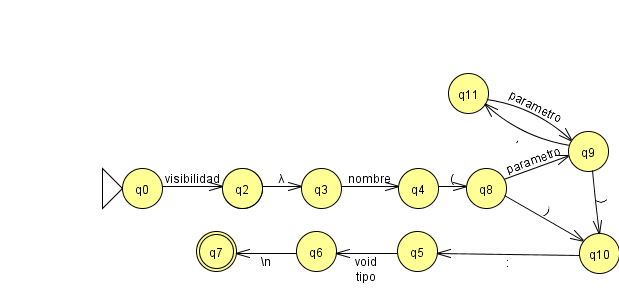
\includegraphics[width=.4\linewidth]{automatas_finitos/metodoDrt.png}
	\caption{Autómata finito - Método}
	\label{fig:metodo_af}
\end{figure}

\begin{figure}[H]
	\centering
	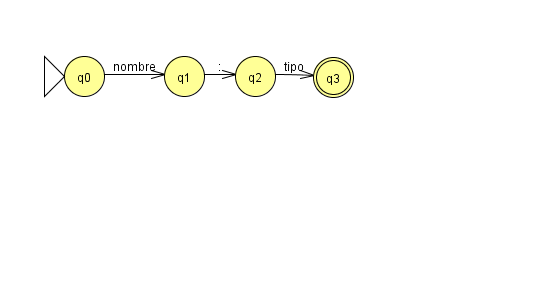
\includegraphics[width=.4\linewidth]{automatas_finitos/parametroDrt.png}
	\caption{Autómata finito - Parámetro}
	\label{fig:metodo_parametro_af}
\end{figure}




\section{Método}
\label{sec:metodo}
Al igual que los atributos, los metodos, son componentes dentro del diagrama de
clases que ayudan a la manipulación de los datos, estos brindan el
comportamiento que es propio al objeto. El lenguaje presentado permite definir
métodos de la siguiente manera:

\begin{lstlisting}[caption={BNF - Método}, basicstyle=\footnotesize\ttfamily]
  <metodo>::=<visibilidad><nombre>"("<parametro>")" ":"<tipo>
  <metodo>::=<visibilidad><nombre>"("<parametros>")" ":"<tipo>
\end{lstlisting}

En donde se puede decir que \texttt{parametro(s)} se define de la siguiente
manera:

\begin{lstlisting}[basicstyle=\footnotesize\ttfamily]
  <parametro> ::= <nombre> ":" <tipo>
\end{lstlisting}

\begin{lstlisting}[basicstyle=\footnotesize\ttfamily]
  <parametros> ::= <parametro> | <parametros>
\end{lstlisting}

Director, está dotado de la capacidad para tratar los casos triviales del
manejo de los datos dentro de un objeto, estos casos triviales corresponden a
situaciones en las cuales una de las necesidades de comportammiento para un
objeto viene dado por la urgencia de agregar algún mecanismo que permita
acceder a los atributos del mismo, las acciones comunes de acceso a estos
atributos son las siguientes: definir el valor de un atributo y obtener el
valor de ese atributo, las cuales son solucionadas con los \texttt{setters}
y los \texttt{getters}.

Director, no requiere que se definan explicitamente estos métodos, éste los
genera de manera automática.

Teniendo en cuenta el ejemplo mencionado en la \texttt{Seccion
\ref{sec:atributo}}, Director automáticamente generaría los siguientes métodos
para el lenguaje Java:

\begin{lstlisting}[language=Java, basicstyle=\footnotesize\ttfamily,
label=lst:drt_java_metodo, caption={Java - Generación \texttt{Fragmento \ref{sec:atributo}}}]
  ...
	public String get_nombre(){
		return this.nombre;
		}

	public void set_nombre(String nombre){
		this.nombre = nombre;
		}

	public String get_apellido(){
		return this.apellido;
		}

	public void set_apellido(String apellido){
		this.apellido = apellido;
		}

	public String get_DNI(){
		return this.DNI;
		}

	public void set_DNI(String DNI){
		this.DNI = DNI;
		}
	...
\end{lstlisting}

De todos modos, es posible indicar otros metodos que se deseen incluir en el
modelo. Si agregaramos algun $metodo\_generico$ al ejemplo con el que se viene
trabajando, la lista de atributos y modelos quedaría definida de la siguiente
manera.

\begin{lstlisting}[caption={Director - Declaración de Método}, label=lst:drt_java_modelo_metodo_generico]
	private nombre:string
	private apellido:string
	private DNI:string
	public metodo_generico():void
\end{lstlisting}

Lo que resultaria en la generación del ``esqueleto'' necesario para la
implementación de dicho método. Tomando como base lo que ya se hizo en
el \texttt{Fragmento \ref{lst:drt_java_metodo}}, se le agregaría:

\begin{lstlisting}[caption={Java - Generación metodo\_generico agregado en
\texttt{Fragmento \ref{lst:drt_java_modelo_metodo_generico}}}, language=Java, basicstyle=\footnotesize\ttfamily]
  public void metodo_generico() {
		// Implementacion del metodo
		}
\end{lstlisting}


\subsection*{Autómatas finitos}
\label{sub:metodo_af}

Aquí se proporcionarán los autómatas finitos para la definición de un método y
las subcomponentes que se crearon para éste, como por ejemplo el
\texttt{parametro}.

\begin{figure}[H]
	\centering
	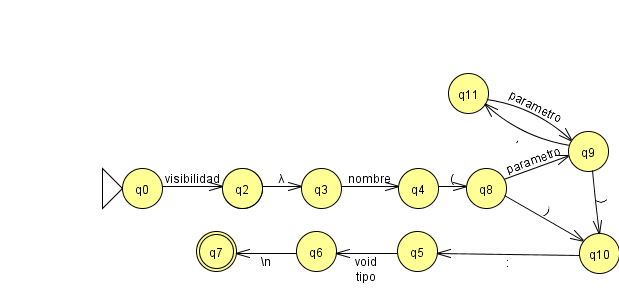
\includegraphics[width=.4\linewidth]{automatas_finitos/metodoDrt.png}
	\caption{Autómata finito - Método}
	\label{fig:metodo_af}
\end{figure}

\begin{figure}[H]
	\centering
	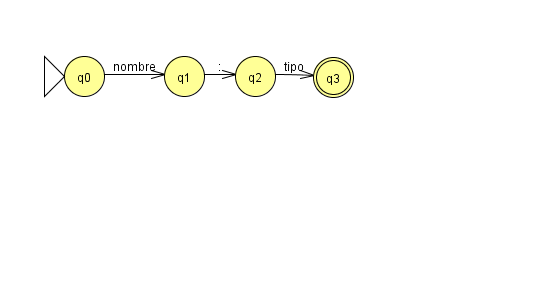
\includegraphics[width=.4\linewidth]{automatas_finitos/parametroDrt.png}
	\caption{Autómata finito - Parámetro}
	\label{fig:metodo_parametro_af}
\end{figure}




\section{Método}
\label{sec:metodo}
Al igual que los atributos, los metodos, son componentes dentro del diagrama de
clases que ayudan a la manipulación de los datos, estos brindan el
comportamiento que es propio al objeto. El lenguaje presentado permite definir
métodos de la siguiente manera:

\begin{lstlisting}[caption={BNF - Método}, basicstyle=\footnotesize\ttfamily]
  <metodo>::=<visibilidad><nombre>"("<parametro>")" ":"<tipo>
  <metodo>::=<visibilidad><nombre>"("<parametros>")" ":"<tipo>
\end{lstlisting}

En donde se puede decir que \texttt{parametro(s)} se define de la siguiente
manera:

\begin{lstlisting}[basicstyle=\footnotesize\ttfamily]
  <parametro> ::= <nombre> ":" <tipo>
\end{lstlisting}

\begin{lstlisting}[basicstyle=\footnotesize\ttfamily]
  <parametros> ::= <parametro> | <parametros>
\end{lstlisting}

Director, está dotado de la capacidad para tratar los casos triviales del
manejo de los datos dentro de un objeto, estos casos triviales corresponden a
situaciones en las cuales una de las necesidades de comportammiento para un
objeto viene dado por la urgencia de agregar algún mecanismo que permita
acceder a los atributos del mismo, las acciones comunes de acceso a estos
atributos son las siguientes: definir el valor de un atributo y obtener el
valor de ese atributo, las cuales son solucionadas con los \texttt{setters}
y los \texttt{getters}.

Director, no requiere que se definan explicitamente estos métodos, éste los
genera de manera automática.

Teniendo en cuenta el ejemplo mencionado en la \texttt{Seccion
\ref{sec:atributo}}, Director automáticamente generaría los siguientes métodos
para el lenguaje Java:

\begin{lstlisting}[language=Java, basicstyle=\footnotesize\ttfamily,
label=lst:drt_java_metodo, caption={Java - Generación \texttt{Fragmento \ref{sec:atributo}}}]
  ...
	public String get_nombre(){
		return this.nombre;
		}

	public void set_nombre(String nombre){
		this.nombre = nombre;
		}

	public String get_apellido(){
		return this.apellido;
		}

	public void set_apellido(String apellido){
		this.apellido = apellido;
		}

	public String get_DNI(){
		return this.DNI;
		}

	public void set_DNI(String DNI){
		this.DNI = DNI;
		}
	...
\end{lstlisting}

De todos modos, es posible indicar otros metodos que se deseen incluir en el
modelo. Si agregaramos algun $metodo\_generico$ al ejemplo con el que se viene
trabajando, la lista de atributos y modelos quedaría definida de la siguiente
manera.

\begin{lstlisting}[caption={Director - Declaración de Método}, label=lst:drt_java_modelo_metodo_generico]
	private nombre:string
	private apellido:string
	private DNI:string
	public metodo_generico():void
\end{lstlisting}

Lo que resultaria en la generación del ``esqueleto'' necesario para la
implementación de dicho método. Tomando como base lo que ya se hizo en
el \texttt{Fragmento \ref{lst:drt_java_metodo}}, se le agregaría:

\begin{lstlisting}[caption={Java - Generación metodo\_generico agregado en
\texttt{Fragmento \ref{lst:drt_java_modelo_metodo_generico}}}, language=Java, basicstyle=\footnotesize\ttfamily]
  public void metodo_generico() {
		// Implementacion del metodo
		}
\end{lstlisting}


\subsection*{Autómatas finitos}
\label{sub:metodo_af}

Aquí se proporcionarán los autómatas finitos para la definición de un método y
las subcomponentes que se crearon para éste, como por ejemplo el
\texttt{parametro}.

\begin{figure}[H]
	\centering
	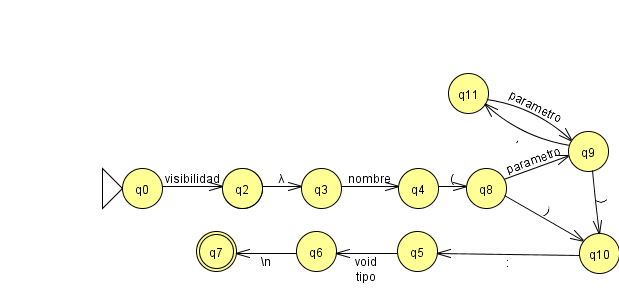
\includegraphics[width=.4\linewidth]{automatas_finitos/metodoDrt.png}
	\caption{Autómata finito - Método}
	\label{fig:metodo_af}
\end{figure}

\begin{figure}[H]
	\centering
	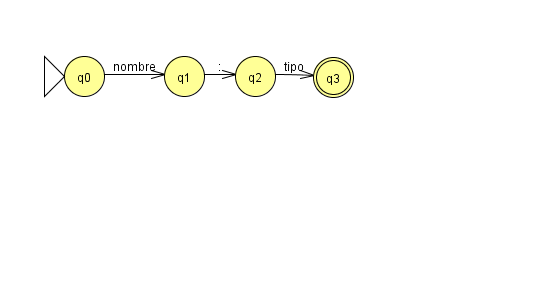
\includegraphics[width=.4\linewidth]{automatas_finitos/parametroDrt.png}
	\caption{Autómata finito - Parámetro}
	\label{fig:metodo_parametro_af}
\end{figure}




\section{Método}
\label{sec:metodo}
Al igual que los atributos, los metodos, son componentes dentro del diagrama de
clases que ayudan a la manipulación de los datos, estos brindan el
comportamiento que es propio al objeto. El lenguaje presentado permite definir
métodos de la siguiente manera:

\begin{lstlisting}[caption={BNF - Método}, basicstyle=\footnotesize\ttfamily]
  <metodo>::=<visibilidad><nombre>"("<parametro>")" ":"<tipo>
  <metodo>::=<visibilidad><nombre>"("<parametros>")" ":"<tipo>
\end{lstlisting}

En donde se puede decir que \texttt{parametro(s)} se define de la siguiente
manera:

\begin{lstlisting}[basicstyle=\footnotesize\ttfamily]
  <parametro> ::= <nombre> ":" <tipo>
\end{lstlisting}

\begin{lstlisting}[basicstyle=\footnotesize\ttfamily]
  <parametros> ::= <parametro> | <parametros>
\end{lstlisting}

Director, está dotado de la capacidad para tratar los casos triviales del
manejo de los datos dentro de un objeto, estos casos triviales corresponden a
situaciones en las cuales una de las necesidades de comportammiento para un
objeto viene dado por la urgencia de agregar algún mecanismo que permita
acceder a los atributos del mismo, las acciones comunes de acceso a estos
atributos son las siguientes: definir el valor de un atributo y obtener el
valor de ese atributo, las cuales son solucionadas con los \texttt{setters}
y los \texttt{getters}.

Director, no requiere que se definan explicitamente estos métodos, éste los
genera de manera automática.

Teniendo en cuenta el ejemplo mencionado en la \texttt{Seccion
\ref{sec:atributo}}, Director automáticamente generaría los siguientes métodos
para el lenguaje Java:

\begin{lstlisting}[language=Java, basicstyle=\footnotesize\ttfamily,
label=lst:drt_java_metodo, caption={Java - Generación \texttt{Fragmento \ref{sec:atributo}}}]
  ...
	public String get_nombre(){
		return this.nombre;
		}

	public void set_nombre(String nombre){
		this.nombre = nombre;
		}

	public String get_apellido(){
		return this.apellido;
		}

	public void set_apellido(String apellido){
		this.apellido = apellido;
		}

	public String get_DNI(){
		return this.DNI;
		}

	public void set_DNI(String DNI){
		this.DNI = DNI;
		}
	...
\end{lstlisting}

De todos modos, es posible indicar otros metodos que se deseen incluir en el
modelo. Si agregaramos algun $metodo\_generico$ al ejemplo con el que se viene
trabajando, la lista de atributos y modelos quedaría definida de la siguiente
manera.

\begin{lstlisting}[caption={Director - Declaración de Método}, label=lst:drt_java_modelo_metodo_generico]
	private nombre:string
	private apellido:string
	private DNI:string
	public metodo_generico():void
\end{lstlisting}

Lo que resultaria en la generación del ``esqueleto'' necesario para la
implementación de dicho método. Tomando como base lo que ya se hizo en
el \texttt{Fragmento \ref{lst:drt_java_metodo}}, se le agregaría:

\begin{lstlisting}[caption={Java - Generación metodo\_generico agregado en
\texttt{Fragmento \ref{lst:drt_java_modelo_metodo_generico}}}, language=Java, basicstyle=\footnotesize\ttfamily]
  public void metodo_generico() {
		// Implementacion del metodo
		}
\end{lstlisting}


\subsection*{Autómatas finitos}
\label{sub:metodo_af}

Aquí se proporcionarán los autómatas finitos para la definición de un método y
las subcomponentes que se crearon para éste, como por ejemplo el
\texttt{parametro}.

\begin{figure}[H]
	\centering
	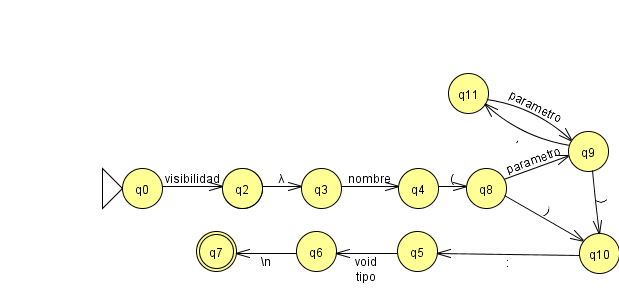
\includegraphics[width=.4\linewidth]{automatas_finitos/metodoDrt.png}
	\caption{Autómata finito - Método}
	\label{fig:metodo_af}
\end{figure}

\begin{figure}[H]
	\centering
	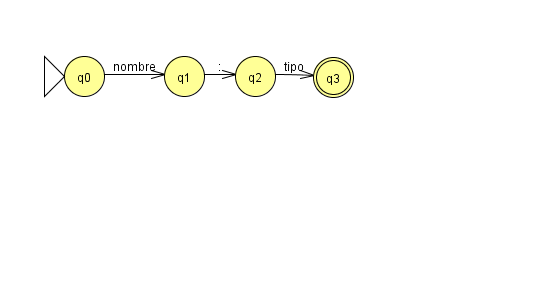
\includegraphics[width=.4\linewidth]{automatas_finitos/parametroDrt.png}
	\caption{Autómata finito - Parámetro}
	\label{fig:metodo_parametro_af}
\end{figure}




\section{Método}
\label{sec:metodo}
Al igual que los atributos, los metodos, son componentes dentro del diagrama de
clases que ayudan a la manipulación de los datos, estos brindan el
comportamiento que es propio al objeto. El lenguaje presentado permite definir
métodos de la siguiente manera:

\begin{lstlisting}[caption={BNF - Método}, basicstyle=\footnotesize\ttfamily]
  <metodo>::=<visibilidad><nombre>"("<parametro>")" ":"<tipo>
  <metodo>::=<visibilidad><nombre>"("<parametros>")" ":"<tipo>
\end{lstlisting}

En donde se puede decir que \texttt{parametro(s)} se define de la siguiente
manera:

\begin{lstlisting}[basicstyle=\footnotesize\ttfamily]
  <parametro> ::= <nombre> ":" <tipo>
\end{lstlisting}

\begin{lstlisting}[basicstyle=\footnotesize\ttfamily]
  <parametros> ::= <parametro> | <parametros>
\end{lstlisting}

Director, está dotado de la capacidad para tratar los casos triviales del
manejo de los datos dentro de un objeto, estos casos triviales corresponden a
situaciones en las cuales una de las necesidades de comportammiento para un
objeto viene dado por la urgencia de agregar algún mecanismo que permita
acceder a los atributos del mismo, las acciones comunes de acceso a estos
atributos son las siguientes: definir el valor de un atributo y obtener el
valor de ese atributo, las cuales son solucionadas con los \texttt{setters}
y los \texttt{getters}.

Director, no requiere que se definan explicitamente estos métodos, éste los
genera de manera automática.

Teniendo en cuenta el ejemplo mencionado en la \texttt{Seccion
\ref{sec:atributo}}, Director automáticamente generaría los siguientes métodos
para el lenguaje Java:

\begin{lstlisting}[language=Java, basicstyle=\footnotesize\ttfamily,
label=lst:drt_java_metodo, caption={Java - Generación \texttt{Fragmento \ref{sec:atributo}}}]
  ...
	public String get_nombre(){
		return this.nombre;
		}

	public void set_nombre(String nombre){
		this.nombre = nombre;
		}

	public String get_apellido(){
		return this.apellido;
		}

	public void set_apellido(String apellido){
		this.apellido = apellido;
		}

	public String get_DNI(){
		return this.DNI;
		}

	public void set_DNI(String DNI){
		this.DNI = DNI;
		}
	...
\end{lstlisting}

De todos modos, es posible indicar otros metodos que se deseen incluir en el
modelo. Si agregaramos algun $metodo\_generico$ al ejemplo con el que se viene
trabajando, la lista de atributos y modelos quedaría definida de la siguiente
manera.

\begin{lstlisting}[caption={Director - Declaración de Método}, label=lst:drt_java_modelo_metodo_generico]
	private nombre:string
	private apellido:string
	private DNI:string
	public metodo_generico():void
\end{lstlisting}

Lo que resultaria en la generación del ``esqueleto'' necesario para la
implementación de dicho método. Tomando como base lo que ya se hizo en
el \texttt{Fragmento \ref{lst:drt_java_metodo}}, se le agregaría:

\begin{lstlisting}[caption={Java - Generación metodo\_generico agregado en
\texttt{Fragmento \ref{lst:drt_java_modelo_metodo_generico}}}, language=Java, basicstyle=\footnotesize\ttfamily]
  public void metodo_generico() {
		// Implementacion del metodo
		}
\end{lstlisting}


\subsection*{Autómatas finitos}
\label{sub:metodo_af}

Aquí se proporcionarán los autómatas finitos para la definición de un método y
las subcomponentes que se crearon para éste, como por ejemplo el
\texttt{parametro}.

\begin{figure}[H]
	\centering
	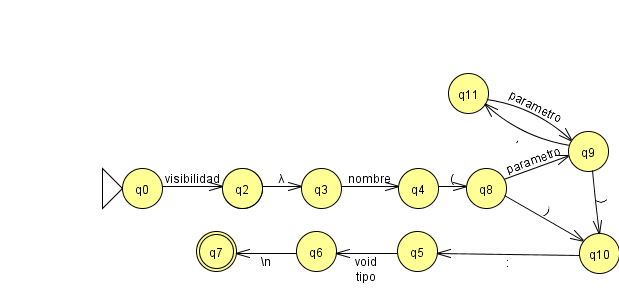
\includegraphics[width=.4\linewidth]{automatas_finitos/metodoDrt.png}
	\caption{Autómata finito - Método}
	\label{fig:metodo_af}
\end{figure}

\begin{figure}[H]
	\centering
	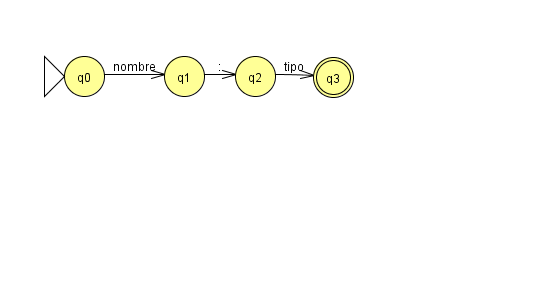
\includegraphics[width=.4\linewidth]{automatas_finitos/parametroDrt.png}
	\caption{Autómata finito - Parámetro}
	\label{fig:metodo_parametro_af}
\end{figure}




\section{Método}
\label{sec:metodo}
Al igual que los atributos, los metodos, son componentes dentro del diagrama de
clases que ayudan a la manipulación de los datos, estos brindan el
comportamiento que es propio al objeto. El lenguaje presentado permite definir
métodos de la siguiente manera:

\begin{lstlisting}[caption={BNF - Método}, basicstyle=\footnotesize\ttfamily]
  <metodo>::=<visibilidad><nombre>"("<parametro>")" ":"<tipo>
  <metodo>::=<visibilidad><nombre>"("<parametros>")" ":"<tipo>
\end{lstlisting}

En donde se puede decir que \texttt{parametro(s)} se define de la siguiente
manera:

\begin{lstlisting}[basicstyle=\footnotesize\ttfamily]
  <parametro> ::= <nombre> ":" <tipo>
\end{lstlisting}

\begin{lstlisting}[basicstyle=\footnotesize\ttfamily]
  <parametros> ::= <parametro> | <parametros>
\end{lstlisting}

Director, está dotado de la capacidad para tratar los casos triviales del
manejo de los datos dentro de un objeto, estos casos triviales corresponden a
situaciones en las cuales una de las necesidades de comportammiento para un
objeto viene dado por la urgencia de agregar algún mecanismo que permita
acceder a los atributos del mismo, las acciones comunes de acceso a estos
atributos son las siguientes: definir el valor de un atributo y obtener el
valor de ese atributo, las cuales son solucionadas con los \texttt{setters}
y los \texttt{getters}.

Director, no requiere que se definan explicitamente estos métodos, éste los
genera de manera automática.

Teniendo en cuenta el ejemplo mencionado en la \texttt{Seccion
\ref{sec:atributo}}, Director automáticamente generaría los siguientes métodos
para el lenguaje Java:

\begin{lstlisting}[language=Java, basicstyle=\footnotesize\ttfamily,
label=lst:drt_java_metodo, caption={Java - Generación \texttt{Fragmento \ref{sec:atributo}}}]
  ...
	public String get_nombre(){
		return this.nombre;
		}

	public void set_nombre(String nombre){
		this.nombre = nombre;
		}

	public String get_apellido(){
		return this.apellido;
		}

	public void set_apellido(String apellido){
		this.apellido = apellido;
		}

	public String get_DNI(){
		return this.DNI;
		}

	public void set_DNI(String DNI){
		this.DNI = DNI;
		}
	...
\end{lstlisting}

De todos modos, es posible indicar otros metodos que se deseen incluir en el
modelo. Si agregaramos algun $metodo\_generico$ al ejemplo con el que se viene
trabajando, la lista de atributos y modelos quedaría definida de la siguiente
manera.

\begin{lstlisting}[caption={Director - Declaración de Método}, label=lst:drt_java_modelo_metodo_generico]
	private nombre:string
	private apellido:string
	private DNI:string
	public metodo_generico():void
\end{lstlisting}

Lo que resultaria en la generación del ``esqueleto'' necesario para la
implementación de dicho método. Tomando como base lo que ya se hizo en
el \texttt{Fragmento \ref{lst:drt_java_metodo}}, se le agregaría:

\begin{lstlisting}[caption={Java - Generación metodo\_generico agregado en
\texttt{Fragmento \ref{lst:drt_java_modelo_metodo_generico}}}, language=Java, basicstyle=\footnotesize\ttfamily]
  public void metodo_generico() {
		// Implementacion del metodo
		}
\end{lstlisting}


\subsection*{Autómatas finitos}
\label{sub:metodo_af}

Aquí se proporcionarán los autómatas finitos para la definición de un método y
las subcomponentes que se crearon para éste, como por ejemplo el
\texttt{parametro}.

\begin{figure}[H]
	\centering
	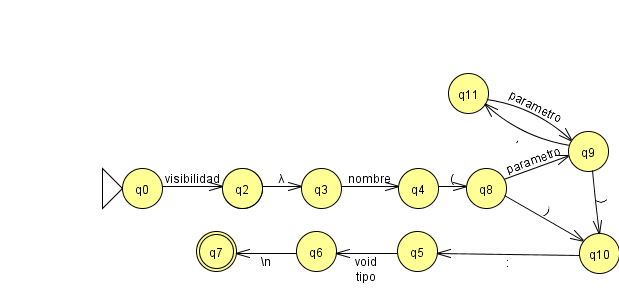
\includegraphics[width=.4\linewidth]{automatas_finitos/metodoDrt.png}
	\caption{Autómata finito - Método}
	\label{fig:metodo_af}
\end{figure}

\begin{figure}[H]
	\centering
	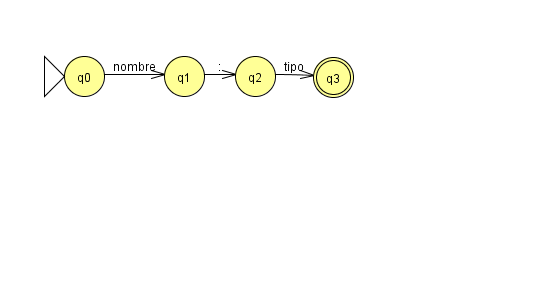
\includegraphics[width=.4\linewidth]{automatas_finitos/parametroDrt.png}
	\caption{Autómata finito - Parámetro}
	\label{fig:metodo_parametro_af}
\end{figure}




\section{Método}
\label{sec:metodo}
Al igual que los atributos, los metodos, son componentes dentro del diagrama de
clases que ayudan a la manipulación de los datos, estos brindan el
comportamiento que es propio al objeto. El lenguaje presentado permite definir
métodos de la siguiente manera:

\begin{lstlisting}[caption={BNF - Método}, basicstyle=\footnotesize\ttfamily]
  <metodo>::=<visibilidad><nombre>"("<parametro>")" ":"<tipo>
  <metodo>::=<visibilidad><nombre>"("<parametros>")" ":"<tipo>
\end{lstlisting}

En donde se puede decir que \texttt{parametro(s)} se define de la siguiente
manera:

\begin{lstlisting}[basicstyle=\footnotesize\ttfamily]
  <parametro> ::= <nombre> ":" <tipo>
\end{lstlisting}

\begin{lstlisting}[basicstyle=\footnotesize\ttfamily]
  <parametros> ::= <parametro> | <parametros>
\end{lstlisting}

Director, está dotado de la capacidad para tratar los casos triviales del
manejo de los datos dentro de un objeto, estos casos triviales corresponden a
situaciones en las cuales una de las necesidades de comportammiento para un
objeto viene dado por la urgencia de agregar algún mecanismo que permita
acceder a los atributos del mismo, las acciones comunes de acceso a estos
atributos son las siguientes: definir el valor de un atributo y obtener el
valor de ese atributo, las cuales son solucionadas con los \texttt{setters}
y los \texttt{getters}.

Director, no requiere que se definan explicitamente estos métodos, éste los
genera de manera automática.

Teniendo en cuenta el ejemplo mencionado en la \texttt{Seccion
\ref{sec:atributo}}, Director automáticamente generaría los siguientes métodos
para el lenguaje Java:

\begin{lstlisting}[language=Java, basicstyle=\footnotesize\ttfamily,
label=lst:drt_java_metodo, caption={Java - Generación \texttt{Fragmento \ref{sec:atributo}}}]
  ...
	public String get_nombre(){
		return this.nombre;
		}

	public void set_nombre(String nombre){
		this.nombre = nombre;
		}

	public String get_apellido(){
		return this.apellido;
		}

	public void set_apellido(String apellido){
		this.apellido = apellido;
		}

	public String get_DNI(){
		return this.DNI;
		}

	public void set_DNI(String DNI){
		this.DNI = DNI;
		}
	...
\end{lstlisting}

De todos modos, es posible indicar otros metodos que se deseen incluir en el
modelo. Si agregaramos algun $metodo\_generico$ al ejemplo con el que se viene
trabajando, la lista de atributos y modelos quedaría definida de la siguiente
manera.

\begin{lstlisting}[caption={Director - Declaración de Método}, label=lst:drt_java_modelo_metodo_generico]
	private nombre:string
	private apellido:string
	private DNI:string
	public metodo_generico():void
\end{lstlisting}

Lo que resultaria en la generación del ``esqueleto'' necesario para la
implementación de dicho método. Tomando como base lo que ya se hizo en
el \texttt{Fragmento \ref{lst:drt_java_metodo}}, se le agregaría:

\begin{lstlisting}[caption={Java - Generación metodo\_generico agregado en
\texttt{Fragmento \ref{lst:drt_java_modelo_metodo_generico}}}, language=Java, basicstyle=\footnotesize\ttfamily]
  public void metodo_generico() {
		// Implementacion del metodo
		}
\end{lstlisting}


\subsection*{Autómatas finitos}
\label{sub:metodo_af}

Aquí se proporcionarán los autómatas finitos para la definición de un método y
las subcomponentes que se crearon para éste, como por ejemplo el
\texttt{parametro}.

\begin{figure}[H]
	\centering
	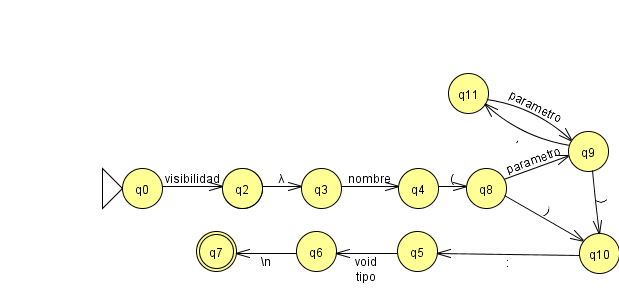
\includegraphics[width=.4\linewidth]{automatas_finitos/metodoDrt.png}
	\caption{Autómata finito - Método}
	\label{fig:metodo_af}
\end{figure}

\begin{figure}[H]
	\centering
	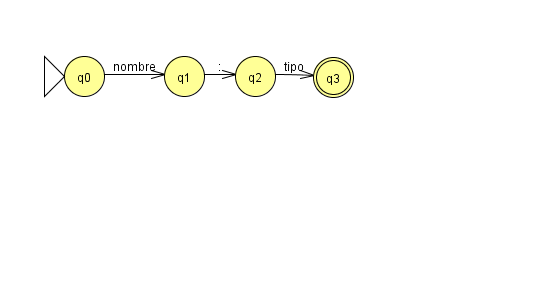
\includegraphics[width=.4\linewidth]{automatas_finitos/parametroDrt.png}
	\caption{Autómata finito - Parámetro}
	\label{fig:metodo_parametro_af}
\end{figure}




